\documentclass[problems]{esg8012pset} 
  \usepackage{amsmath}
  \usepackage{amssymb}
  \usepackage{enumerate}
  \usepackage{graphicx}
  \providecommand{\uvec}[1]{{\hat{\bf{#1}}}}
  \usepackage{pgf,tikz}
  \usetikzlibrary{arrows}
  \makeatletter
  \newcommand{\interitemtext}[1]{%
    \begin{list}{}
     {\itemindent=0mm\labelsep=0mm
     \labelwidth=0mm\leftmargin=0mm
     \addtolength{\leftmargin}{-\@totalleftmargin}}
      \item #1
    \end{list}
  }
  \makeatother
  \renewcommand{\d}{\,d}
  \providecommand{\norm}[1]{\lVert#1\rVert}
\classname{Physics 8.012} 
\semester{Fall 2010} 
\problemsetnumber{3} 
\date{September 24} 
\duedate{Friday, October 1} 
\readingassignment{Kleppner and Kolenkow, \emph {An Introduction to Mechanics}, Chapter Two} 
\begin{document}
\section*{Problem 1: K\&K 2.24}
  A device called a capstan is used aboard ships in order to control a rope which is under great tension. The rope is wrapped around a fixed drum, usually for several turns (the drawing shows about three fourths turn). The load on the rope pulls it with a force $T_A$, and the sailor holds it with a much smaller force $T_B$.  Can you show that $T_B = T_Ae^{-\mu_s\theta}$, where $\mu_s$ is the coefficient of static friction and $\theta$ is the total angle subtended by the rope on the drum?
  \begin{center}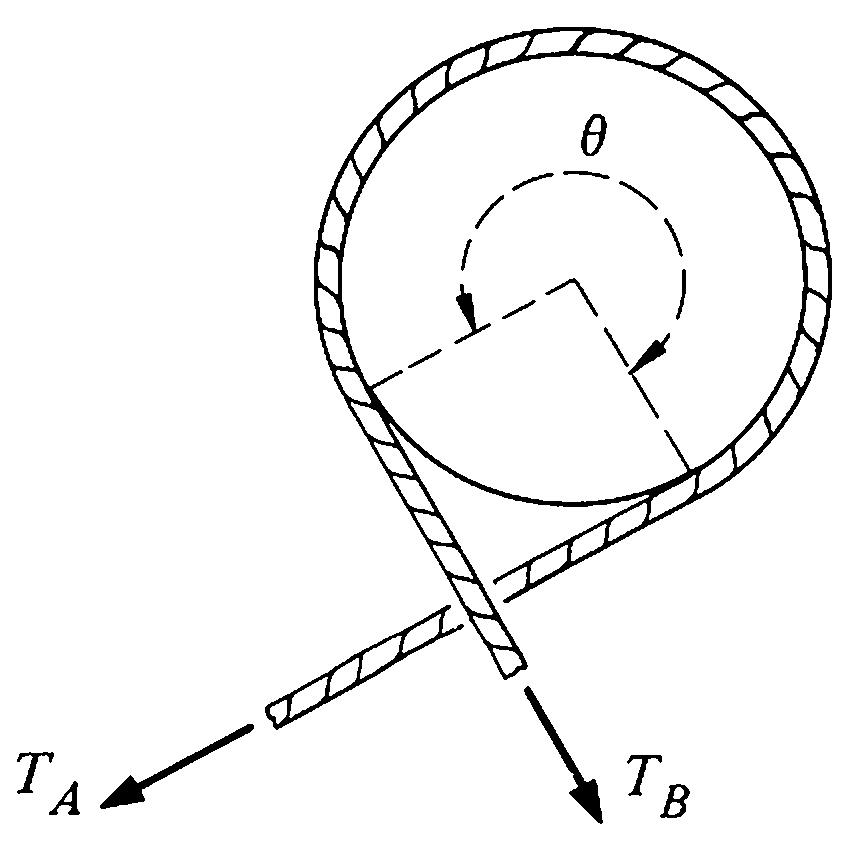
\includegraphics[width=0.35\textwidth]{ps03_1}\end{center}
